
\subsection{Double Integrals}

\BEN 
% ~~~~~~~~~~~~~~~~~~~~~~~~~~~~~~~~~~~~~~~~~~~~~~~~~~~~~~~~~~~~~~~~~~~~~~~~~~~~~~~~~
\item % VOLUME OF SIMPLE SOLID 
\BEN
\item A sketch of the volume is below. 
\begin{figure}[h]
  \vspace{-1pt}
  \begin{center}
    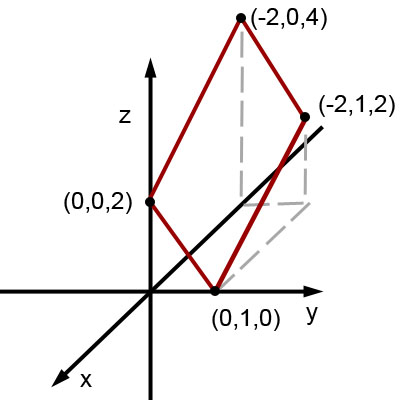
\includegraphics[width=0.35\textwidth]{ImgSolid.jpg}
  \end{center}
\end{figure}
\item We must integrate:
\begin{align*}
  \mathop{\int_{-2}^0 \! \int_0^1} (-x-2y+2 ) dydx 
  &= \int_{-2}^0 \big( -2xy -y^2 + 2y \big) \big|_0^1 dx \\
  &= \int_{-2}^0 \Big( -2x + 1  \Big) dx \\
  &= \Big(-x^2 + x \Big) \Big|_{-2}^0  \\  
  &= 0- \big(- (-2)^2 + (-2)\big)\\
  &= 0- \big(- 4 -2\big)\\
  &= 6
\end{align*}
\EEN
% ~~~~~~~~~~~~~~~~~~~~~~~~~~~~~~~~~~~~~~~~~~~~~~~~~~~~~~~~~~~~~~~~~~~~~~~~~~~~~~~~~
\item % FLUID MECHANICS
\BEN
\item Substituting the expression for $u$ into the divergence equation yields
\begin{align*}
  0&= \nabla \cdot \MB{v} \\
  &= \px \big(u(x,y)\big) + \py \big(v(x,y)\big) \\
  &= \px (x^2 + y^2) + \frac{\partial v}{\partial y}\\
  &= 2x + \frac{\partial v}{\partial y} \\
   \frac{\partial v}{\partial y} &= -2x 
\end{align*}
Therefore, $v(x,y)$ is a function whose partial derivative with respect to $y$ is $-2x$. The \Emph{most general} form for $v(x,y)$ is obtained by integrating with respect to $y$:
\begin{align*}
 v(x,y) &= -2xy + f(x)
\end{align*}
where $f(x)$ is an unknown function of one variable, $x$. 
\item Using the same approach as we used for (a) yields
\begin{align*}
  0&= \nabla \cdot \MB{v} \\
  &= \px \big(u(x,y)\big) + \py \big(v(x,y)\big) \\
  &=  \frac{\partial u}{\partial x}+ 0\\
   \frac{\partial u}{\partial x} &= 0
\end{align*}
Therefore, $u(x,y)$ is a function whose partial derivative with respect to $x$ is $0$. The \Emph{most general} form for $u(x,y)$ is obtained by integrating with respect to $x$:
\begin{align*}
 u(x,y) &= g(y)
\end{align*}
where $g(y)$ is an unknown function of one variable, $y$. 
\EEN
% ~~~~~~~~~~~~~~~~~~~~~~~~~~~~~~~~~~~~~~~~~~~~~~~~~~~~~~~~~~~~~~~~~~~~~~~~~~~~~~~~~
\item % INTEGRAL WITH AN ABSOLUTE VALUE
\textbf{Double Integral with an Absolute Value}\\
We are given the double integral
\begin{align*}
  \mathop{\int_{0}^{1} \! \int_0^{2}  }y \big| x-1\big| dxdy.
\end{align*}
Treating $y$ as a constant, this becomes
\begin{align*}
  \int_{0}^{1} y \Bigg( \int_0^{2}   \big| x-1\big| dx\Bigg)dy.
\end{align*}
and we must then evaluate 
\begin{align*}
  \int_0^{2}   \big| x-1\big| dx.
\end{align*}
The absolute value function can be removed if we note that 
\begin{align*}
|x - 1| = \left\{
\begin{array}{rl}
1-x & \text{if } x \le 1\\
x-1 & \text{if } x > 1\\
\end{array} \right.
\end{align*}
Thus, 
\begin{align*}
  \int_0^{2}   \big| x-1\big| dx 
  &=  \int_0^{2}   \big| x-1\big| dx \\
  &=  \int_0^{1}   \big| x-1\big| dx +  \int_1^{2}   \big| x-1\big| dx \\
  &=  \int_0^{1}  ( 1 - x ) dx +  \int_1^{2}   (x - 1) dx \\
  &=  1 - \frac{1}{2} +    \Big(\frac{x^2}{2} - x\Big)\Big|_1^{2} \\
  &=  \frac{1}{2} +    \Big((2-2) - (1/2-1)\Big) \\
  &=  \frac{1}{2} +    \Big(0 - (-1/2)\Big) \\
  &=  \frac{1}{2} + \frac{1}{2}\\
  &= 1
\end{align*}
Therefore,
\begin{align*}
  \int_{0}^{1} y \Bigg( \int_0^{2}   \big| x-1\big| dx\Bigg)dy =   \int_{0}^{1} y (1) dy =   \frac{y^2}{2}\Big|_{0}^{1}= \frac{1}{2} .
\end{align*}
Note that the integral 
\begin{align*}
  \int_0^{2}   \big| x-1\big| dx.
\end{align*}
is simply the area of two triangles, each with area $\frac{1}{2}$. So a much simpler method of working out the answer to the integral with respect to $x$ is 
\begin{align*}
  \int_0^{2}   \big| x-1\big| dx = \frac{1}{2} + \frac{1}{2} = 1.
\end{align*}
% ~~~~~~~~~~~~~~~~~~~~~~~~~~~~~~~~~~~~~~~~~~~~~~~~~~~~~~~~~~~~~~~~~~~~~~~~~~~~~~~~~
\item % MAXIMUM AND MINIMUM VALUES
\textbf{Double Integral Given Maximum and Minimum Values}\\
If the maximum and minimum values of $f(x,y)$ on $S$ are equal to the constant $K$, then $f(x,y)$ is constant on $S$, and is equal to $K$ everywhere on $S$. 
Then,
\begin{align*}
  \iint\limits_S f(x,y) dxdy = \mathop{\int_{a}^{b} \! \int_c^{d}  } K dxdy  = K \mathop{\int_{a}^{b} \! \int_c^{d}  } (1) dxdy = K(b-a)(d-c).
\end{align*}

\EEN % END OF SUBSECTION
%\newpage
%% s~s~s~s~s~s~s~s~s~s~s~s~s~s~s~s~s~s~s~s~s~s~s~s~s~s~s~s~s~s~s~s~s~s~s~s~s~s~s~s~s~s~s~s
%\subsection{Double Integrals Over a General Region}
%\BEN
%% ~~~~~~~~~~~~~~~~~~~~~~~~~~~~~~~~~~~~~~~~~~~~~~~~~~~~~~~~~~~~~~~~~~~~~~~~~~~~~~~~~
%\item % TETRAHEDRON
%\BEN
%\item A sketch of the tetrahedron is below. 
%\begin{figure}[h]
%  \vspace{-1pt}
%  \begin{center}
%    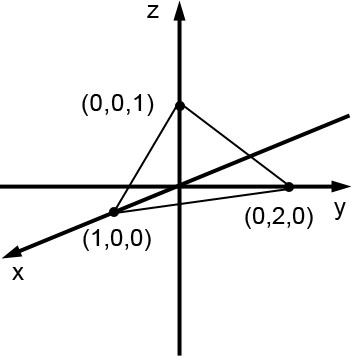
\includegraphics[width=0.35\textwidth]{ImgTetExample.jpg}
%  \end{center}
%\end{figure}
%% ~  ~  ~  ~  ~  ~  ~  ~  ~  ~  ~  ~  ~  ~  ~  ~  ~  ~  ~  ~  ~  ~  ~  ~  
%\item The tetrahedron has one side in the $xy$-plane. This side is bounded by the line that is the intersection between the $xy$-plane and the plane $z = 1 - x - y/2$. We can find this intersection by setting $z=0$,
%\begin{align*}
%  0 &= 1 - x - \frac{y}{2} \\
%  x &= 1 - \frac{y}{2}.
%\end{align*}
%Therefore, the volume is the region under the plane $z = 1 - x - y/2$ and over  
%\begin{align*}
%  R = \{ (x,y) \ | \ 0 \le x \le 1- y/2, \ 0 \le y \le 2 \}.
%\end{align*}
%The double integral is 
%\begin{align*}
%  \mathop{\int_{0}^{2} \! \int_0^{1-y/2} } (1 - x - \frac{y}{2}) dxdy
%\end{align*} 
%% ~  ~  ~  ~  ~  ~  ~  ~  ~  ~  ~  ~  ~  ~  ~  ~  ~  ~  ~  ~  ~  ~  ~  ~  
%\item The volume is the region under the plane $z = 1 - x - y/2$ and over  
%\begin{align*}
%  R = \{ (x,y) \ | \ 0 \le x \le 1, \ 0 \le y \le 2 - 2x \}.
%\end{align*}
%The double integral is 
%\begin{align*}
%  \mathop{\int_{0}^{1} \! \int_0^{2-2x} } (1 - x - \frac{y}{2}) dydx
%\end{align*} 
%\EEN
%% ~~~~~~~~~~~~~~~~~~~~~~~~~~~~~~~~~~~~~~~~~~~~~~~~~~~~~~~~~~~~~~~~~~~~~~~~~~~~~~~~~
%\item % DOUBLE INTEGRAL IS AREA IF F=1
%\BEN
%\item
%Suppose that we subdivide region $R$ into a rectangular grid of sub-rectangles (as in Figure 3.2.5), so that we only consider the sub-rectangles that are completely enclosed in $R$. Then, the area of region $R$ is approximated by the double sum
%\begin{align*}
%  \sum_j\sum_i\Delta x_i \Delta y_j
%\end{align*}
%But if $f=1$ for all $x_i$ and $y_j$, this is equal to:
%\begin{align}\label{abefaberabreabr}
%  \sum_j\sum_i f(x_i,y_j) \Delta x_i \Delta y_j
%\end{align}
%where $x_i$ and $y_j$ is a point inside sub-rectangle $[x_i,x_{i+1}]\times[y_j,y_{j+1}]$. 
%If we take smaller and smaller rectangles, so that the length of the longest diagonal of the sub-rectangles goes to zero, the sub-rectangles begin to fill more and more of the region $R$, and so the above sums approach the  \Emph{area} of region $R$. Since we have defined
%\begin{align*}
%  \mathop{\int \!\!\! \int} f(x,y) dA
%\end{align*}
%as the limit of Equation (\ref{abefaberabreabr}) as the longest diagonal goes to zero, and $f(x,y)=1$, the double integral 
%\begin{align*}
%  \mathop{\int \!\!\! \int} 1 dA
%\end{align*}
%is the area of region $R$. 
%\item The region may be defined as
%\begin{align*}
%  R = \{ (x,y) \ | \ 0 \le x \le 1, \ x^2 \le y \le \sqrt{x} \}.
%\end{align*}
%The area of $R$ is 
%\begin{align*}
%  \mathop{\int_0^1 \!\!\! \int_{x^2}^{\sqrt{x}}} dydx 
%  &= \int_0^1 \Big(\sqrt{x} - x^2 \Big) dx \\
%  &= \Big(\frac{2}{3}x^{3/2}  - \frac{x^3}{3} \Big)\Big|_0^1 \\
%  &= \frac{2}{3} - \frac{1}{3} \\
%  &= \frac{1}{3}
%\end{align*}
%\EEN
%% ~~~~~~~~~~~~~~~~~~~~~~~~~~~~~~~~~~~~~~~~~~~~~~~~~~~~~~~~~~~~~~~~~~~~~~~~~~~~~~~~~
%\item % UPPER AND LOWER BOUNDS ARE FUNCTIONS
%The curves $y=x^2$ and $x^2=y$ intersect at (0,0) and at (1,1). Integrating with respect to $y$ first yields
%\begin{align*} 
%  \mathop{\int_0^1 \!\!\! \int_{x^2}^{\sqrt{x}}} x^2+y^2 dydx 
%  &= \int_0^1 \Big(yx^2 + \frac{y^3}{3} \Big)\Big|_{x^2}^{\sqrt{x}} dx \\
%  &= \int_0^1 \Big(x^{5/2} + \frac{x^{3/2}}{3} - x^4 - \frac{x^6}{3}\Big) dx \\
%  &= \Big( \frac{2}{7} x^{7/2} + \frac{2}{15}x^{5/2} - \frac{1}{5}x^5 - \frac{1}{21}x^7\Big)\Big|_0^1 \\
%  &= \frac{2}{7} + \frac{2}{15} - \frac{1}{5} - \frac{1}{21} \\
%  &= 6/35
%\end{align*}
%% ~~~~~~~~~~~~~~~~~~~~~~~~~~~~~~~~~~~~~~~~~~~~~~~~~~~~~~~~~~~~~~~~~~~~~~~~~~~~~~~~~
%\item % CHANGING ORDER OF INTEGRATION
%\BEN 
%\item Integrating with respect to $y$ first yields
%\begin{align*} 
%  \mathop{\int_0^2 \!\!\! \int_0^{x^2}} x\sin (y) dydx 
%  &= \int_0^2 -x\cos(y)\Big|_0^{x^2} dx \\
%  &= - \int_0^2 \Big(x\cos(x^2)-1\Big) dx \\
%  &= - \int_0^2x\cos(x^2) dx +  \int_0^2 1 \ dx \\    
%  &= 2 - \int_0^2x\cos(x^2) dx 
%\end{align*}
%Now let $u=x^2$, so that $du = 2xdx$. Then 
%\begin{align*} 
%  2 - \int_0^2x\cos(x^2) dx  
%  &=  2 - \int_0^4 x\cos(u)\Big(\frac{du}{2x}\Big)\\
%  &=  2 - \frac{1}{2} \int_0^4 \cos(u)du \\
%  &=  2 - \frac{1}{2} \sin(u) \Big|_0^4 \\
%  &=  2 - \frac{1}{2} \sin(4) \\
%  &\approx 2.3784
%\end{align*}
%\item Integrating with respect to $x$ first yields
%\begin{align*} 
%  \mathop{\int_0^4 \!\!\! \int_{\sqrt{y}}^{2} } x\sin (y) dxdy
%  &= \int_0^4 \frac{x^2}{2}\sin(y)\Big|_{\sqrt{y}}^{2} \ dy \\
%  &= \int_0^4 \frac{4-y}{2}\sin(y) dy \\
%  &= 2 \int_0^4 \sin(y) dy - \frac{1}{2} \int_0^4 y\sin(y) dy \\
%  &= 2 \big( - \cos(y) \big)\big|_0^4 - \frac{1}{2} \int_0^4 y\sin(y) dy \\
%  &= 2 \big( - \cos(4) + 1 \big) - \frac{1}{2} \int_0^4 y\sin(y) dy \\
%  &= 2  - 2\cos(4)  - \frac{1}{2} \int_0^4 y\sin(y) dy \\
%\end{align*}
%Now using integration by parts, with 
%\begin{align*}
%  u &= y, \quad dv = \sin(y)dy \\
%  du &= dy, \quad v = -\cos(y)
%\end{align*}
%we obtain
%\begin{align*} 
%  \mathop{\int_0^4 \!\!\! \int_{\sqrt{y}}^{2} } x\sin (y) dxdy
%  &= 2  - 2\cos(4)  - \frac{1}{2} \int_0^4 y\sin(y) dy \\
%  &= 2  - 2\cos(4)  - \frac{1}{2}\Bigg( -y\cos(y)\Big|_0^4 - \int_0^4 \big(-\cos(y)\big) dy \Bigg) \\
%  &= 2  - 2\cos(4)  - \frac{1}{2}\Bigg( -4\cos4 + \sin(y)\big|_0^4 \Bigg)  \\  
%  &= 2  - 2\cos(4)  - \frac{1}{2}\Big( -4\cos4 + \sin(4)- 0 \Big)  \\  
%  &= 2 - \frac{\sin(4)}{2}   \\  
%  &\approx 2.3784
%\end{align*}
%\EEN
%% ~~~~~~~~~~~~~~~~~~~~~~~~~~~~~~~~~~~~~~~~~~~~~~~~~~~~~~~~~~~~~~~~~~~~~~~~~~~~~~~~~
%\item % CHANGING ORDER OF INTEGRATION, GENERAL F(X,Y)
%The region over which we are integrating $f(x,y)$ is the shaded area below. 
%\begin{figure}[h]
%  \vspace{-1pt}
%  \begin{center}
%    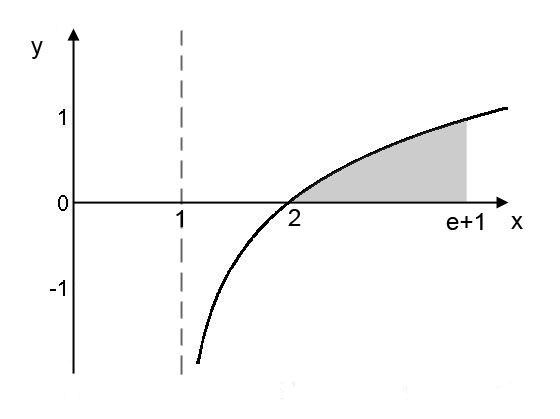
\includegraphics[width=0.55\textwidth]{ImgLog.jpg}
%  \end{center}
%\end{figure}\\
%The region is bounded by the lines $y=0$, $x=1+e$, and by the curve $y=\ln(x-1)$. Using horizontal slices, values of $y$ range from 0 to 1, and values of $x$ range from $e^y-1$ to $1+e$. The double integral becomes
%\begin{align*}
%  \mathop{\int_{0}^{1} \! \int_{e^y-1}^{1+e}} f(x,y) dydx .
%\end{align*}
%% ~~~~~~~~~~~~~~~~~~~~~~~~~~~~~~~~~~~~~~~~~~~~~~~~~~~~~~~~~~~~~~~~~~~~~~~~~~~~~~~~~
%\item % BOUNDING AN INTEGRAL 
%The integrand $f(x,y)$ has the property that 
%\begin{align*}
%  0 \le \sin(x+y) \le 1,
%\end{align*}
%because $x+y$ is between 0 and 2, and $\sin(2) < 1$. Then 
%\begin{align*}
%  0 = \iint\limits_D 0 dA  \le  \iint\limits_D f(x,y) dA \le  \iint\limits_D (1) dA = 1.
%\end{align*}
%% ~~~~~~~~~~~~~~~~~~~~~~~~~~~~~~~~~~~~~~~~~~~~~~~~~~~~~~~~~~~~~~~~~~~~~~~~~~~~~~~~~
%\item % SYMMETRY
%\BEN
%\item 
%Suppose we use the function
%\begin{align*}
% h(x,y) & = 11xy.
%\end{align*}
%Then $h(-x,y) = 11(-x)y = -11xy = -h(x,y)$. 
%\item An example of a region that is symmetric about the $y$-axis, but not symmetric about the $x$-axis, is the region bounded by the curves
%\begin{align*}
%  x = -1,  \quad x = 1, \quad y = 0, \quad y = - 1.
%\end{align*}
%\item The double integral for our region is
%\begin{align*}
%  \iint\limits_D g(x,y) dxdy 
%  &=  \mathop{\int_{-1}^1 \! \int_{-1}^0} 11xy dydx\\
%  &=  -\frac{11}{2} \int_{-1}^1 x dx\\
%  &=  -\frac{11}{4} \Big(x^2 \Big)\Big|_{-1}^{1} \\
%  &=  -\frac{11}{4} (0)\\
%  &= 0.
%\end{align*}
%\EEN
%% ~~~~~~~~~~~~~~~~~~~~~~~~~~~~~~~~~~~~~~~~~~~~~~~~~~~~~~~~~~~~~~~~~~~~~~~~~~~~~~~~~
%\EEN % END OF SOLUTIONS
%\newpage
%% s~s~s~s~s~s~s~s~s~s~s~s~s~s~s~s~s~s~s~s~s~s~s~s~s~s~s~s~s~s~s~s~s~s~s~s~s~s~s~s~s~s~s~s
%% s~s~s~s~s~s~s~s~s~s~s~s~s~s~s~s~s~s~s~s~s~s~s~s~s~s~s~s~s~s~s~s~s~s~s~s~s~s~s~s~s~s~s~s
%\subsection{Triple Integrals}
%
%\BEN
%% ~~~~~~~~~~~~~~~~~~~~~~~~~~~~~~~~~~~~~~~~~~~~~~~~~~~~~~~~~~~~~~~~~~~~~~~~~~~~~~~~~
%\item % TETRAHEDRON
%\Emph{Volume of a Tetrahedron} \\
%\begin{figure}[h]
%  \vspace{-1pt}
%  \begin{center}
%    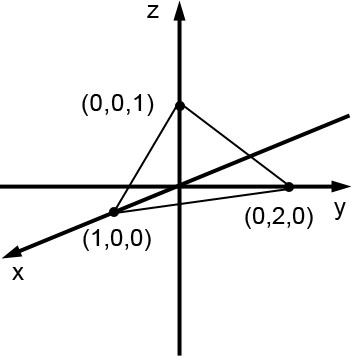
\includegraphics[width=0.35\textwidth]{ImgTetExample.jpg}
%  \end{center}
%\end{figure}\\
%Recall that the volume is the region under the plane $z = 1 - x - y/2$ and over  
%\begin{align*}
%  R = \{ (x,y) \ | \ 0 \le x \le 1- y/2, \ 0 \le y \le 2 \}.
%\end{align*}
%Because $z$ lies between 0 and $z = 1 - x - y/2$, the volume, $S$, can be described as
%\begin{align*}
%  S = \{ (x,y,z) \ | \ 0 \le x \le 1- y/2, \ 0 \le y \le 2, \ 0 \le z \le 1 - x - y/2 \}.
%\end{align*}
%The volume can be calculated with the triple integral
%\begin{align*}
%  \mathop{\int_{0}^{2} \! \int_0^{1-y/2} \int_0^{1-x-y/2} }dzdxdy
%  &= \mathop{\int_{0}^{2} \! \int_0^{1-y/2}  } ( 1-x-y/2) dxdy\\
%  &= \mathop{\int_{0}^{2}  } \Big( x-\frac{x^2}{2}-\frac{xy}{2}\Big)\Big|_0^{1-y/2} dy \\
%  &= \mathop{\int_{0}^{2}  } \Big( (1-y/2)-\frac{(1-y/2)^2}{2}-\frac{(y-y^2/2)}{2}\Big) dy \\
%  &= \mathop{\int_{0}^{2}  } \Bigg( 1 - \frac{y}{2}-\frac{1}{2}\Big(1 - y + \frac{y^2}{4}\Big)-\frac{y}{2}+\frac{y^2}{4}\Bigg) dy \\
%  &= \mathop{\int_{0}^{2}  } \Bigg( 1 - \frac{y}{2} - \frac{1}{2} + \frac{y}{2} - \frac{y^2}{8} -\frac{y}{2}+\frac{y^2}{4}\Bigg) dy \\
%  &= \mathop{\int_{0}^{2}  } \Big( \frac{1}{2} - \frac{y}{2} + \frac{y^2}{8} \Big) dy \\
%  &= \frac{2}{2} - \frac{4}{4}  + \frac{8}{24} \\
%  &= \frac{1}{3}
%\end{align*} 
%% ~~~~~~~~~~~~~~~~~~~~~~~~~~~~~~~~~~~~~~~~~~~~~~~~~~~~~~~~~~~~~~~~~~~~~~~~~~~~~~~~~
%\item % VOLUME OF AN ELLIPSOID
%\textbf{Volume of an Ellipsoid}\\
%We are given the transformations  
%\begin{align*}
%  x=au, \quad y=bv, \quad z=cw.
%\end{align*}
%The Jacobian becomes 
%\begin{align*}   J &=  
%  \begin{vmatrix}
%   \pxu &  \pxv & \pxw \\\\
%   \pyu & \pyv & \pyw \\\\
%   \pzu & \pzv & \pzw 
%  \end{vmatrix}
%  =     
%  \begin{vmatrix}
% a&0&0\\
% 0&b&0\\
% 0&0&c\\
%  \end{vmatrix}
%  = abc.
% \end{align*}
% The solid enclosed by the ellipsoid is the image of the unit sphere $u^2 + v^2 + w^2 \le 1$. Using that a sphere has volume $\frac{4}{3} \pi r^3$, we find that 
%\begin{align*}
%  \iiint\limits_{V} dxdydz
%  &=  \iiint\limits_{u^2+v^2+w^2 \le 1} abc \ dudvdw \\
%  &=  abc \iiint\limits_{u^2+v^2+w^2 \le 1} \ dudvdw \\
%  &=  abc (\text{volume of a sphere}) \\
%  &=   \frac{4\pi abc}{3} 
%\end{align*}
%
%% ~~~~~~~~~~~~~~~~~~~~~~~~~~~~~~~~~~~~~~~~~~~~~~~~~~~~~~~~~~~~~~~~~~~~~~~~~~~~~~~~~
%\item % MAXIMIZING A TRIPLE INTEGRAL
%\textbf{Maximizing a Triple Integral}\\
%The integral will obtain its maximum value when $S$ contains the entire region where the integrand is non-negative. In other words, we require that 
%\begin{align*}
%  1 - 3x^2 - 2y^2 - 4z^2 \ge 0 .
%\end{align*}
%Therefore, $E$ is the region bounded by the ellipse
%\begin{align*}
%   3x^2 + 2y^2 + 4z^2 = 1.
%\end{align*}
%% ~~~~~~~~~~~~~~~~~~~~~~~~~~~~~~~~~~~~~~~~~~~~~~~~~~~~~~~~~~~~~~~~~~~~~~~~~~~~~~~~~
%\EEN % END OF SUBSECTION
%% s~s~s~s~s~s~s~s~s~s~s~s~s~s~s~s~s~s~s~s~s~s~s~s~s~s~s~s~s~s~s~s~s~s~s~s~s~s~s~s~s~s~s~s
%% s~s~s~s~s~s~s~s~s~s~s~s~s~s~s~s~s~s~s~s~s~s~s~s~s~s~s~s~s~s~s~s~s~s~s~s~s~s~s~s~s~s~s~s
%\subsection{Change of Variables in Multiple Integrals}
%
%\BEN
%% ~~~~~~~~~~~~~~~~~~~~~~~~~~~~~~~~~~~~~~~~~~~~~~~~~~~~~~~~~~~~~~~~~~~~~~~~~~~~~~~~~
%\item % GENERAL LINEAR TRANSFORMATION
%\Emph{Linear Transformations} \\
%\BEN
%\item Substituting $v = v_0$ into the linear transformation yields the two equations
%\begin{align*}
%  x &= c_1u + c_2v_0 \\ 
%  y &= d_1u + d_2v_0
%\end{align*}
%To find the equation of the line in the $xy$-plane, we need to eliminate $u$. There are many ways to do this, but let's multiply the first equation by $d_1$ and the second by $c_1$.
%\begin{align*}
%  d_1x &= c_1d_1u + c_2d_1v_0 \\ 
%  c_1y &= c_1d_1u + d_2c_1v_0
%\end{align*}
%Subtracting these equations yields
%\begin{align*}
%  d_1x -  c_1y &=  (c_2d_1 -  d_2c_1)v_0 
%\end{align*}
%A simple rearrangement gives us
%\begin{align*}
%  c_1y &= d_1x - (c_2d_1 -  d_2c_1)v_0 .
%\end{align*}
%Provided that $c_1$ is not zero, we could write this in the form
%\begin{align*}
%  y &= \frac{d_1}{c_1}x - \frac{c_2d_1 -  d_2c_1}{c_1}v_0 .
%\end{align*}
%% ~  ~  ~  ~  ~  ~  ~  ~  ~  ~  ~  ~  ~  ~  ~  ~  ~  ~  ~  ~  ~  ~  ~  ~  ~  ~  ~  ~
%\item 
%Substituting $x=x_0$ into $x =c_1u + c_2v$ gives us 
%\begin{align*}
%  x_0 &= c_1u + c_2v,
%\end{align*}
%Provided that $c_2$ is not zero, 
%This is the is mapped into the $uv$-plane REWORD
%\EEN
%
%% ~~~~~~~~~~~~~~~~~~~~~~~~~~~~~~~~~~~~~~~~~~~~~~~~~~~~~~~~~~~~~~~~~~~~~~~~~~~~~~~~~
%\item % STRAIGHTFORWARD CHANGE OF VARIABLES
%\Emph{Double Integral Over a Parallelogram} \\
%The integral can be written as
%\begin{align*}
%  \iint\limits_R \big(x^2 - y^2\big) dxdy =  \iint\limits_R (x - y)(x+y) dxdy.
%\end{align*}
%Recall that $R$ is the region bounded by
%\begin{align*}
%  x+y = 0, \quad x+y = 1, \quad x-y=0, \quad x-y=1.
%\end{align*}
%The appearance of the terms $(x+y)$ and $(x - y)$ in the integrand and in the lines that bound $R$ suggests the transformation 
%\begin{align}
%  u & = x+y  \label{zcvzcxvvad}\\
%  v &= x - y \label{ntrsraaewvbernst}.
%\end{align}
%In order to compute the Jacobian, we need explicit expressions for $u$ and $v$. If we add  equations \ref{zcvzcxvvad} and \ref{ntrsraaewvbernst} we find that 
%\begin{align*}   x = \frac{u+v}{2}   \end{align*}
%And if we subtract equations \ref{zcvzcxvvad} and \ref{ntrsraaewvbernst} we find that
%\begin{align*}   y = \frac{u-v}{2}   \end{align*}
%The Jacobian becomes
%\begin{align*}   J &=  
%  \begin{vmatrix}
%   \pxu &  \pxv \\ \\
%   \pyu & \pyv \\
%  \end{vmatrix}
%  =     \begin{vmatrix}
% \frac{1}{2} &  \frac{1}{2} \\ \\
%   \frac{1}{2} & -\frac{1}{2} \\
%  \end{vmatrix}
%  = - \frac{1}{4}- \frac{1}{4} = - \frac{1}{2}.
% \end{align*}
%We also need to find the limits of  integration in the transformed integral. Using equations \ref{zcvzcxvvad} and \ref{ntrsraaewvbernst} the four lines bounding $R$ in the $xy$-plane become 
%\begin{align*}
%  u = 0, \quad u = 1, \quad v=0, \quad v=1.
%\end{align*}
%The double integral therefore becomes
%\begin{align*}
%  \iint\limits_R \big(x^2 - y^2\big) dxdy 
%  &=  \iint\limits_R (x - y)(x+y) dxdy \\
%  &=    \mathop{\int_0^1 \! \int_0^1} uv \Bigg|-\frac{1}{2} \Bigg| dudv \\
%  &=     \frac{1}{2}\mathop{\int_0^1 \! \int_0^1} (uv) dudv \\
%  &=     \frac{1}{2}\int_0^1 \frac{v}{2} dv \\
%  &=   \frac{1}{8}.
%\end{align*}
%% ~~~~~~~~~~~~~~~~~~~~~~~~~~~~~~~~~~~~~~~~~~~~~~~~~~~~~~~~~~~~~~~~~~~~~~~~~~~~~~~~~
%\item % SIMPLIFYING
%\Emph{Simplifying a Double Integral as a Product of Two Single Integrals} \\
%Substituting $f(x,y) = g(x)h(y)$ into the double integral yields
%\begin{align*}
%   \iint\limits_{R} f(x,y) dA 
%   =  \int_a^b  \int_c^d g(x) h(y) dydx 
%   =  \int_a^b \Bigg( \int_c^d g(x) h(y) dy \Bigg) dx .
%\end{align*}
%The function $g(x)$ is a constant in the inner integral, so
%\begin{align*}
%   \iint\limits_{R} f(x,y) dA 
%   &=  \int_a^b  \Bigg( g(x)\int_c^d h(y) dy \Bigg) dx \\
%   &=  \int_a^b   g(x) \Bigg(\int_c^d h(y) dy \Bigg) dx .
%\end{align*}
%The term in the brackets is a constant, and so 
%\begin{align*}
%   \iint\limits_{R} f(x,y) dA 
%   &=  \int_a^b   g(x) \Bigg(\int_c^d h(y) dy \Bigg) dx \\
%   &=  \int_a^b   g(x) dx \int_c^d h(y) dy.
%\end{align*}
%This is the result we were asked to prove.
%% ~~~~~~~~~~~~~~~~~~~~~~~~~~~~~~~~~~~~~~~~~~~~~~~~~~~~~~~~~~~~~~~~~~~~~~~~~~~~~~~~~
%\item % 
%\Emph{Triple Integral Bounded by an Ellipse} \\
%The Jacobian is
%\begin{align*}   J &=  
%  \begin{vmatrix}
%   \pxu &  \pxv \\ \\
%   \pyu & \pyv \\
%  \end{vmatrix}
%  =     \begin{vmatrix}
%   3 & 0 \\ \\
%   0 & 2 \\
%  \end{vmatrix}
%  = 6 .
% \end{align*}
%We also need to find the limits of integration in the transformed integral. The region $R$ is bounded by the ellipse, $4x^2 + 9y^2 = 36$, which becomes the region bounded by the circle $u^2 + v^2 = 1$. Therefore
%\begin{align*}
%  \iint\limits_R x^2 \ dxdy &= \iint\limits_{u^2 + v^2 \le 1} (9u^2) 6dudv =  54 \iint\limits_{u^2 + v^2 \le 1} (u^2) dudv
%\end{align*}
%Switching to polar coordinates, 
%\begin{align*}
%  u = r\cos\theta, \quad v = r\sin\theta, \quad J = r
%\end{align*}
%our double integral becomes
%\begin{align*}
%  54 \iint\limits_{u^2 + v^2 \le 1} (u^2) dudv 
%  & = 54 \mathop{\int_0^{2\pi} \!\! \int_0^1} r^3\cos^2\theta drd\theta  \\
%  & = 54 \Bigg( \int_0^{2\pi} \cos^2\theta d\theta \Bigg)\Bigg( \int_0^1 r^3 dr \Bigg) \\
%  & = 54 \Bigg( \int_0^{2\pi} \frac{1}{2} \big(1+\cos(2\theta) \big) d\theta \Bigg) \Bigg( \frac{1}{4} \Bigg) \\
%  & =\frac{27}{4} \Bigg( \int_0^{2\pi}  \big(1+\cos(2\theta) \big) d\theta \Bigg) \\
%  & =\frac{27}{4} \big(\theta+\frac{1}{2}\sin(2\theta) \big|_0^{2\pi}  \\
%  & =\frac{27}{4} \big(2\pi\big)  \\
%  & =\frac{27\pi}{2} 
%\end{align*}
%% ~~~~~~~~~~~~~~~~~~~~~~~~~~~~~~~~~~~~~~~~~~~~~~~~~~~~~~~~~~~~~~~~~~~~~~~~~~~~~~~~~
%\item % SIMPLE CYLINDRICAL WITH CONE
%In cylindrical coordinates, the region is described by 
%\begin{align*}
%  V = \{(r,\theta,z) \ | \ 0 \le r \le 1, 0 \le \theta \le 2\pi, 0 \le z \le 3r \}.
%\end{align*}
%Our integral becomes 
%\begin{align*}
%  \iiint\limits_V (r\sin\theta)^2 rdzdrd\theta 
%  &=    \mathop{\int_0^{2\pi} \!\! \int_0^1  \!\! \int_0^{3r}} r^3\sin^2\theta dzdrd\theta  \\
%  &=   3 \mathop{\int_0^{2\pi} \!\! \int_0^1} r^4\sin^2\theta drd\theta  \\
%  &=   \frac{3}{5} \int_0^{2\pi} \sin^2\theta d\theta  \\
%  &=   \frac{3}{10} \int_0^{2\pi} \big(1 - \cos(2\theta)\big) d\theta  \\
%  &=   \frac{3}{10} \big(\theta - \frac{1}{2}\sin(2\theta)\big) \Big|_0^{2\pi} \\
%  &=   \frac{3\pi}{5}
%\end{align*}
%% ~~~~~~~~~~~~~~~~~~~~~~~~~~~~~~~~~~~~~~~~~~~~~~~~~~~~~~~~~~~~~~~~~~~~~~~~~~~~~~~~~
%\item % TRIPLE INTEGRAL IN CYLINDRICAL COORDINATES
%In cylindrical coordinates,  $V$ is the region bounded by
%\begin{align*}
%  0 \le\ &r \le 2 \\
%  0 \le\ &\theta \le \frac{\pi}{2}\\
%  0 \le\ &z \le \sqrt{4 - r^2}
%\end{align*}
%The triple integral becomes
%\begin{align*}
%  \iiint\limits_V dxdydz
%  &=    \mathop{\int_0^{\pi/2} \!\! \int_0^2  \!\! \int_0^{\sqrt{4 - r^2}}} r dzdrd\theta  \\
%  &=    \mathop{\int_0^{\pi/2} \!\! \int_0^2 } r\sqrt{4 - r^2}drd\theta  \\
%  &=   \frac{-1}{3} \int_0^{\pi/2} (4 - r^2)^{3/2} \Big|_0^2 d\theta  \\
%  &=   \frac{-1}{3} \int_0^{\pi/2} (0 - 8) d\theta  \\
%  &=   \frac{4\pi}{3}
%\end{align*}
%% ~~~~~~~~~~~~~~~~~~~~~~~~~~~~~~~~~~~~~~~~~~~~~~~~~~~~~~~~~~~~~~~~~~~~~~~~~~~~~~~~~
%\item % TRIPLE INTEGRAL IN SPHERICAL COORDINATES
%\Emph{Triple Integral In Spherical Coordinates} \\
%The solid is a section of a sphere with radius 1, centered at the origin. The section is the part of the sphere that lies above the plane $z=0$, and between the planes $y=0$, and $y=x$. 
%\begin{align*}
%  \mathop{\int_0^{\pi/4} \!\! \int_{0}^{\pi/2} \!\! \int_0^1 } ( \rho^2 \sin\phi ) \ d\rho\  d\phi\  d\theta
%  &=   \mathop{\int_0^{\pi/4} \!\! \int_{0}^{\pi/2} }  \frac{ \sin\phi}{3}  d\phi\  d\theta\\
%  &=   \int_0^{\pi/4} \frac{-(0-1)}{3}   d\theta \\
%  &=  \pi/12
%\end{align*}
%% ~~~~~~~~~~~~~~~~~~~~~~~~~~~~~~~~~~~~~~~~~~~~~~~~~~~~~~~~~~~~~~~~~~~~~~~~~~~~~~~~~
%\EEN % END OF SUBSECTION
%% s~s~s~s~s~s~s~s~s~s~s~s~s~s~s~s~s~s~s~s~s~s~s~s~s~s~s~s~s~s~s~s~s~s~s~s~s~s~s~s~s~s~s~s
%% s~s~s~s~s~s~s~s~s~s~s~s~s~s~s~s~s~s~s~s~s~s~s~s~s~s~s~s~s~s~s~s~s~s~s~s~s~s~s~s~s~s~s~s
%\subsection{Application: Center of Mass}
%\BEN
%% ~~~~~~~~~~~~~~~~~~~~~~~~~~~~~~~~~~~~~~~~~~~~~~~~~~~~~~~~~~~~~~~~~~~~~~~~~~~~~~~~~
%\item % CENTER OF MASS OF 2D TRIANGULAR PLATE
%\Emph{Center of Mass of a 2D Triangular Plate} \\
%The total mass of the plate is
%\begin{align*}
%  M 
%  &= \iint\limits_R \delta(x,y) dA \\
%  &=    \mathop{\int_0^1 \!\! \int_{2x}^{4x} } xy \ dydx \\
%  &=  \frac{1}{2}  \int_0^1 x(16x^2 - 4x^2) \ dx \\
%  &= 6  \int_0^1 x^3 \ dx \\
%  &=   \frac{3}{2}.
%\end{align*}
%
%The $x$-coordinate of the center of mass is
%\begin{align*}
%  \bar{x} = \frac{M_y}{M} 
%  &= \frac{2}{3} \iint\limits_R x \delta(x,y) dA \\
%  &=    \mathop{\int_0^1 \!\! \int_{2x}^{4x} } x^2y \ dydx \\
%  &=  \frac{1}{2}  \int_0^1 x^2(16x^2 - 4x^2) \ dx \\
%  &= 6  \int_0^1 x^4 \ dx \\
%  &=   \frac{6}{5}.
%\end{align*}
%
%The $y$-coordinate of the center of mass is
%\begin{align*}
%  \bar{y} = \frac{M_x}{M} 
%  &= \frac{2}{3} \iint\limits_R y \delta(x,y) dA \\
%  &=    \mathop{\int_0^1 \!\! \int_{2x}^{4x} } xy^2 \ dydx \\
%  &=  \frac{1}{3}  \int_0^1 x(64x^3 - 8x^3) \ dx \\
%  &=  \frac{56}{3}  \int_0^1 x^4 \ dx \\
%  &=   \frac{56}{15}.
%\end{align*}
%Thus, the coordinates of the center of mass are $(6/5,56/15)$.
%% ~~~~~~~~~~~~~~~~~~~~~~~~~~~~~~~~~~~~~~~~~~~~~~~~~~~~~~~~~~~~~~~~~~~~~~~~~~~~~~~~~
%\item % CENTER OF MASS OF 2D RADIAL DENSITY FUNCTION
%\Emph{Center of Mass of a 2D Plate, Radial Density Function} \\
%We could express the coordinates of the center of mass using either Cartesian or polar coordinates. Using Cartesian coordinates, the density, $\delta$, at point $(x,y)$, is given by
%\begin{align*}
%  \delta(x,y) = L(x,y) = a - \sqrt{x^2+y^2}.
%\end{align*}
%\BEN
%\item
%The $x$-coordinate of the center of mass is
%\begin{align*}
%  \bar{x} = \frac{M_y}{M} 
%  = \frac{1}{M} \iint\limits_R x \delta(x,y) dA 
%  = \frac{1}{M}  \mathop{\int_{-a}^{a} \!\! \int_{0}^{\sqrt{x^2+y^2}}} x\Big( a - \sqrt{x^2+y^2}\Big) \ dydx 
%\end{align*}
%\item
%The $y$-coordinate of the center of mass is
%\begin{align*}
%  \bar{y} = \frac{M_x}{M} 
%  = \frac{1}{M} \iint\limits_R y \delta(x,y) dA 
%  = \frac{1}{M}  \mathop{\int_{-a}^{a} \!\! \int_{0}^{\sqrt{x^2+y^2}}} y\Big( a - \sqrt{x^2+y^2}\Big) \ dydx 
%\end{align*}
%\item The center of mass is located on the $y$-axis. In other words, $\bar{x}=0$. This is because of symmetry: the integrand of $\bar{x}$ is odd in $x$, the integral with respect to $x$ is calculated about an interval that is symmetric about the $y$-axis, and so the integral with respect to $x$ is zero. 
%\EEN
%Note that we could just as easily set up the above integrals using polar coordinates. The 2D circular plate, in polar coordinates, is bounded by 
%\begin{align*}
%  0 \le r \le a, \quad 0 \le \theta \le \pi, \quad a > 0.
%\end{align*}
%The coordinates for the center of mass are
%\begin{align*}
%  \bar{x} &= \frac{M_y}{M} 
%  = \frac{1}{M} \iint\limits_R x \delta(x,y) dA 
%  = \frac{1}{M}  \mathop{\int_{0}^{\pi} \!\! \int_{0}^r} r\cos(\theta) ( a - r ) \ rdrd\theta \\
%  \bar{y} &= \frac{M_x}{M} 
%  = \frac{1}{M} \iint\limits_R y \delta(x,y) dA 
%  = \frac{1}{M}  \mathop{\int_{0}^{\pi} \!\! \int_{0}^r} r\sin(\theta) ( a -r ) \ rdrd\theta
%\end{align*}
% 
%% ~~~~~~~~~~~~~~~~~~~~~~~~~~~~~~~~~~~~~~~~~~~~~~~~~~~~~~~~~~~~~~~~~~~~~~~~~~~~~~~~~
%\item % EVEN AND ODD
%The integral can be written as
%\begin{align*}
%  \mathop{\int_0^{\pi} \!\! \int_{-1}^1} e^{x^2 + y^2}\sin(y) dydx 
%  &= \mathop{\int_0^{\pi} \!\! \int_{-1}^1} e^{x^2}e^{y^2}\sin(y) dydx  = \Bigg( \int_0^{\pi} e^{x^2} dx \Bigg)\Bigg( \int_{-1}^1 e^{y^2}\sin(y)dy \Bigg)  
%\end{align*}
%The second term is the integral of an odd function over a symmetrical interval, and so is equal to zero. Therefore,
%\begin{align*}
%  \mathop{\int_0^{\pi} \!\! \int_{-1}^1} e^{x^2 + y^2}\sin(y) dydx =0.
%\end{align*}
%
%% ~~~~~~~~~~~~~~~~~~~~~~~~~~~~~~~~~~~~~~~~~~~~~~~~~~~~~~~~~~~~~~~~~~~~~~~~~~~~~~~~~
%
%
%
%% ~~~~~~~~~~~~~~~~~~~~~~~~~~~~~~~~~~~~~~~~~~~~~~~~~~~~~~~~~~~~~~~~~~~~~~~~~~~~~~~~~
%\item % CHANGING ORDER OF INTEGRATION
%\rednote{This is a good midterm question}\\
%\textbf{Changing the Order of Integration}\\
%Noting that the limits of integration are not dependent on $y$, the $z$ and the $y$ integrals can be interchanged:
%\begin{align*}
%  V &= \mathop{\int_{0}^{1} \!\! \int_{-\sqrt{x}}^{\sqrt{x}} \! \int_0^{1-x} } dz\ dy\ dx \\
%   &= \mathop{\int_{0}^{1} \Bigg( \int_{-\sqrt{x}}^{\sqrt{x}} dy \Bigg) \Bigg( \int_0^{1-x} } dz\Bigg) dx \\
%   &= \mathop{\int_{0}^{1}  \Bigg( \int_0^{1-x} } dz\Bigg) \Bigg( \int_{-\sqrt{x}}^{\sqrt{x}} dy \Bigg)dx \\
%   &= \mathop{\int_{0}^{1} \!\! \int_0^{1-x} \!\! \int_{-\sqrt{x}}^{\sqrt{x}}} dy\ dz\ dx 
%\end{align*}
%We can also integrate $y$ last. We are given that the solid can be expressed as the region 
%\begin{align*}
%  S = \{(x,y,z)\ |\  0 \le x \le 1, -\sqrt{x} \le y \le \sqrt{x}, 0 \le z \le 1-x \}.
%\end{align*}
%We can re-write this as
%\begin{align*}
%  S = \{(x,y,z)\ |\  y^2 \le x \le 1, -1 \le y \le 1, 0 \le z \le 1-x \}.
%\end{align*}
%This gives us the integral
%\begin{align*}
%  V &= \mathop{\int_{-1}^{1} \! \int_{y^2}^{1} \! \int_0^{1-x} } dz\ dx\ dy
%\end{align*}
%We can also define the region in this way \rednote{wrong}
%\begin{align*}
%  S = \{(x,y,z)\ |\  0 \le x \le 1-z, -1 \le y \le 1, 0 \le z \le 1 \}.
%\end{align*}
%This gives us the integral
%\begin{align*}
%  V &= \mathop{\int_{-1}^{1} \! \int_{0}^{1} \! \int_0^{1-z} } dx\ dz\ dy
%\end{align*}
%
%\EEN % END OF SOLUTIONS
